\documentclass[a4paper]{article}

\usepackage[T2A]{fontenc}
\usepackage[russian]{babel}
\usepackage{graphicx}
\usepackage{float}
\usepackage{hyperref}
\usepackage{amsmath, amssymb, diffcoeff, mathtools}
\usepackage{caption}
\usepackage{geometry}
\usepackage{pdfpages}
\usepackage{wrapfig}

\begin{document}

\begin{center}
\textsc{Санкт-Петербургский национальный исследовательский институт информационных технологий, механики и оптики\\[3mm]
Физический факультет} \\[3mm]

\end{center}
\vspace{5mm}
\line(1,0){\textwidth}
\begin{center}
\textbf{ЛАБОРАТОРНАЯ РАБОТА №2.2\\}
\textbf{"Определение отношения теплоемкостей
воздуха при постоянных давлении и объеме"}
\end{center}
\vspace{2mm}
\line(1,0){\textwidth}
\vspace{5mm}
\begin{minipage}{0.4\textwidth}
    Группа: Z3144 \\
    Студент: Турчанин Евгений\\
    \vspace{1mm}
\end{minipage}
\hfill
\vspace{1mm}
\line(1,0){\textwidth}
1. Изучение процессов в идеальных газах.

2. Определение показателя адиабаты \(\gamma = \frac{C_P}{C_V}\).

\subsection*{Задачи}
1. Измерить значения избыточных давлений в баллоне.

2. Рассчитать отношения теплоемкостей при постоянном давлении и постоянном объеме.

\subsection*{Введение}
Удельной теплоемкостью вещества называется величина \(c\), равная количеству теплоты, которое необходимо сообщить единице массы вещества для изменения ее температуры на один кельвин:

\[
c = \frac{\delta Q}{m \, dT},
\]


где \(\delta Q\) – количество теплоты, сообщенное веществу при нагревании на \(dT\), \(m\) – масса вещества. Единица измерения удельной теплоемкости в системе СИ – Дж/(кг·К).

Молярной теплоемкостью вещества называется физическая величина \(C\), равная количеству теплоты, которое необходимо сообщить одному молю вещества для изменения его температуры на один кельвин:

\[
C = \mu c = \frac{\delta Q}{\nu \, dT},
\]


где \(\mu\) — молярная масса вещества, \(\nu = \frac{m}{\mu}\) — количество вещества. Единица измерения молярной теплоемкости – Дж/(моль·К).

% Страница 3
Численное значение теплоемкости газа зависит от условий его нагревания и количества атомов в его молекуле и ее пространственной конфигурации. В соответствии с первым законом термодинамики:

\[
\delta Q = dU + \delta A.
\]


Увеличение внутренней энергии идеального газа:

\[
dU = \frac{i}{2} \nu R \, dT,
\]


где \(R\) – универсальная газовая постоянная, \(i\) — число степеней свободы молекулы. Для одноатомной молекулы \(i = 3\), для двухатомной жесткой молекулы \(i = 5\), для нелинейной молекулы \(i = 6\).

% Страница 4
При расширении газ выполняет работу:

\[
\delta A = P \, dV.
\]


Молярная теплоемкость \(C_V\) при постоянном объеме:

\[
C_V = \frac{1}{\nu} \left( \frac{\partial U}{\partial T} \right)_V = \frac{i}{2} R.
\]


Молярная теплоемкость \(C_P\) при постоянном давлении:

\[
C_P = C_V + R.
\]


\subsection*{}
Отношение теплоемкостей:

\[
\gamma = \frac{C_P}{C_V} = \frac{i + 2}{i}.
\]


% Страница 5
Адиабатный процесс описывается уравнением:

\[
PV^\gamma = \text{const}.
\]


% Страница 6
Метод Клемана-Дезорма:

\[
(P_0 + P'')V_{\text{min}}^\gamma = P_0 V_{\text{max}}^\gamma,
\]


\[
(P_0 + P'')V_{\text{min}} = (P_0 + P')V_{\text{max}}.
\]


После преобразований:

\[
\gamma = \frac{H}{H - h}.
\]


% Страница 7
\subsection*{Экспериментальная установка}
\begin{figure}[H]
\begin{center}
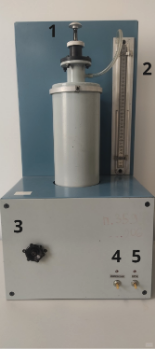
\includegraphics[width=0.5\textwidth]{fig_1}
\caption{ Процессы изменения состояния газа: \\
1 → 2 – адиабатный, 2 → 3 – изохорный, 3 → 1 – изотермический.
}
\end{center}
\end{figure}


\section{Обработка результатов}

\subsection{Расчёт показателя адиабаты}
Показатель адиабаты \(\gamma\) рассчитывается для каждого измерения по формуле:
\[
\gamma = \frac{H}{H - h}
\]
где \(H\) и \(h\) — разности уровней жидкости в манометре до и после адиабатического расширения (в метрах). Результаты измерений и расчётов представлены в таблице:

\begin{table}[h!]
\centering
\caption{Результаты измерений и расчётов}
\begin{tabular}{|c|c|c|c|c|}
\hline
№ & \(H\), м & \(h\), м & \(\gamma\) \\ \hline
1  & 0.019 & 0.002  & 1.118 \\ \hline
2  & 0.015 & 0.002  & 1.154 \\ \hline
3  & 0.025 & 0.000  & 1.000 \\ \hline
4  & 0.021 & 0.001  & 1.050 \\ \hline
5  & 0.018 & -0.001 & 1.056 \\ \hline
6  & 0.015 & 0.000  & 1.000 \\ \hline
7  & 0.019 & 0.000  & 1.000 \\ \hline
8  & 0.021 & 0.001  & 1.050 \\ \hline
9  & 0.024 & -0.001 & 1.042 \\ \hline
10 & 0.020 & 0.000  & 1.000 \\ \hline
\end{tabular}
\end{table}

\subsection{Среднее значение и погрешности}
Среднее значение показателя адиабаты:
\[
\langle \gamma \rangle = \frac{1}{10} \sum_{i=1}^{10} \gamma_i = 1.047
\]

Относительная погрешность рассчитывается по формуле:
\[
\frac{\Delta \gamma}{\gamma} = \frac{H}{H - h} \sqrt{\left( \frac{\Delta H}{H} \right)^2 + \left( \frac{\Delta h}{h} \right)^2}
\]
где \(\Delta H = \Delta h = 0.005 \, \text{м}\) — погрешность измерения уровней. Абсолютная погрешность:
\[
\Delta \gamma = \langle \gamma \rangle \cdot \frac{\Delta \gamma}{\gamma} = 1.047 \cdot 0.012 = 0.013
\]

\subsection{Сравнение с теоретическим значением}
Теоретическое значение показателя адиабаты для воздуха (\(i = 5\) степеней свободы):
\[
\gamma_{\text{теор}} = \frac{i + 2}{i} = \frac{5 + 2}{5} = 1.4
\]

\subsection{Выводы}
В ходе лабораторной работы был проведён эксперимент по определению показателя адиабаты \(\gamma\) для воздуха методом Клемана-Дезорма. Полученные результаты показали, что среднее значение \(\langle \gamma \rangle = 1.047\) с погрешностью \(\Delta \gamma = 0.013\), что отличается от теоретического \(\gamma_{\text{теор}} = 1.4\). Это расхождение может быть вызвано:
\begin{itemize}
    \item Недостаточный временем ожидания до установления равновесия
    \item Ошибкой в расчетах $\gamma$
\end{itemize}

\end{document}

